\documentclass{article}
\usepackage{amsmath,graphicx}
\usepackage{subcaption}
\usepackage{xcolor}

\begin{document}

With $\mu_x$, $\mu_y$ and $\sigma_x^2$, $\sigma_y^2$ being the averages and variances of pixel values along dimensions $x$ and $y$ respectively, $\sigma_{xy}$ being the covariance along $x$ and $y$, $L$ being the dynamic range, $c_1$ and $c_2$, and $c_3$ being defined to be $(k_1L)^2$, $(K_2L)^2$ and $c_2/2$ repectively, with $k_1=0.01$ and $k_2=0.03$, the three components of SSIM metric: luminance $l$, contrast $c$ and structure $s$ are defined as: 

\begin{equation}
l(x,y) = \frac{2\mu_x\mu_y + c_1}{\mu_x^2 + \mu_y^2 + c_1}
\end{equation}

\begin{equation}
  c(x,y) = \frac{2\sigma_x\sigma_y + c_2}{\sigma_x^2 + \sigma_y^2 + c_2}
\end{equation}

\begin{equation}
  s(x,y) = \frac{\sigma_{xy} + c_3}{\sigma_x\sigma_y + c_3}
\end{equation}

Fianlly, SSIM is defined as

\begin{equation}
  SSIM = \frac{1}{n}\sum_x\sum_y [l(x,y)^\alpha. c(x,y)^\beta. s(x,y)^\gamma],
\end{equation}

where $n$ denotes the total number of pixels. The coefficients $\alpha$, $\beta$ and $\gamma$ are generally set to $1$ but are adjustable to suit the application goal.



%--------------------------------okra data-------------------------------
\begin{figure}
    \begin{subfigure}[b]{0.19\linewidth}
        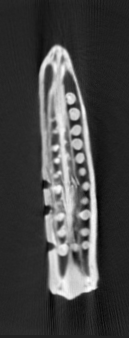
\includegraphics[width=\textwidth]{../images/thesis/okra/templateCropped_1.png}
\captionsetup{labelformat=empty}       
 \caption{}
    \end{subfigure}
    \begin{subfigure}[b]{0.19\linewidth}
        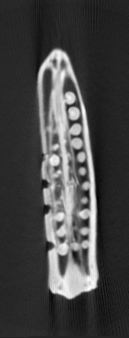
\includegraphics[width=\textwidth]{../images/thesis/okra/templateCropped_2.png}
\captionsetup{labelformat=empty}
        \caption{}
     \end{subfigure}
    \begin{subfigure}[b]{0.19\linewidth}
        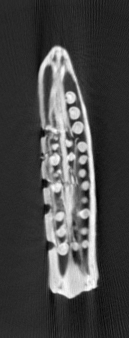
\includegraphics[width=\textwidth]{../images/thesis/okra/templateCropped_3.png}
\captionsetup{labelformat=empty}
        \caption{}
     \end{subfigure}
    \begin{subfigure}[b]{0.19\linewidth}
        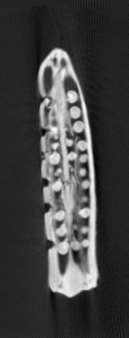
\includegraphics[width=\textwidth]{../images/thesis/okra/templateCropped_4.png}
\captionsetup{labelformat=empty}
        \caption{}
     \end{subfigure}
    \begin{subfigure}[b]{0.186\linewidth}
        \fcolorbox{yellow}{yellow}{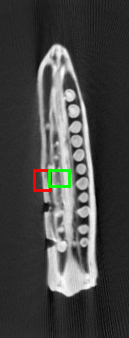
\includegraphics[width=\textwidth]{../images/thesis/okra/testCropped.png}}
\captionsetup{labelformat=empty}
        \caption{}
     \end{subfigure}
     \caption[Okra 3D dataset]{Okra 3D dataset: One slice each from the templates (the
       first four from the left), and one from the test volume
       (extreme right). In the regions marked in red and green, while
       all slices have deformities, the test
       has none.}
\label{fig:templates_test_okra}
\end{figure}
%----------------------------------------------------

\begin{figure}[!h]
\centering
\subcaptionbox{Test}{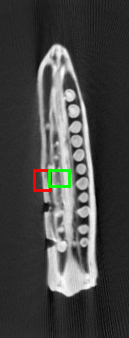
\includegraphics[width=0.19\columnwidth]{../images/thesis/okra/testCropped.png}}\hfill
\subcaptionbox{FDK}{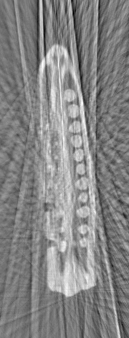
\includegraphics[width=0.19\columnwidth]{../images/thesis/okra/fdk_cropped.png}}\hfill
\subcaptionbox{Sparsity prior}{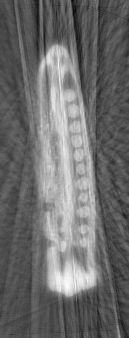
\includegraphics[width=0.19\columnwidth]{../images/thesis/okra/cs_cropped.png}}\hfill
\subcaptionbox{Sparsity and \\unweighted \\template priors}{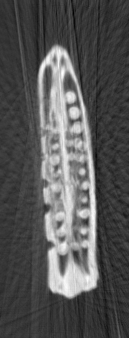
\includegraphics[width=0.19\columnwidth]{../images/thesis/okra/pca_cropped.png}}\hfill
\subcaptionbox{Sparsity and \\weighted template\\ priors}{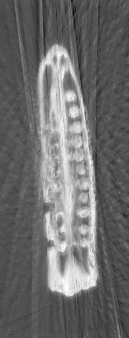
\includegraphics[width=0.19\columnwidth]{../images/thesis/okra/prior_weighted_cropped.png}}
\caption[3D reconstruction of okra dataset]{3D reconstruction of the okra from $10\%$ projection
  views (b) has strong streak artefacts, (c) blurred, (d) no new
  information detected (prior dominates -- the deformity from the prior
  shows up as a false positive) and (e) new information detected (no deformities
  corresponding to red and green regions) while simultaneously
  reducing streak artefacts.}
\label{fig:okra_3D_results}
\end{figure}

%--------------------------------------zoomed okra

\begin{figure}[!h]
\centering
\subcaptionbox{Test}{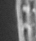
\includegraphics[width=0.19\columnwidth]{../images/thesis/okra/zoomed/input_cropped.png}}\hfill
\subcaptionbox{FDK}{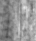
\includegraphics[width=0.19\columnwidth]{../images/thesis/okra/zoomed/FDK_cropped.png}}\hfill
\subcaptionbox{Sparsity prior}{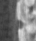
\includegraphics[width=0.19\columnwidth]{../images/thesis/okra/zoomed/pca_cropped.png}}\hfill
\subcaptionbox{Sparsity and \\unweighted \\template priors}{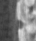
\includegraphics[width=0.19\columnwidth]{../images/thesis/okra/zoomed/pca_cropped.png}}\hfill
\subcaptionbox{Sparsity and \\weighted template\\ priors}{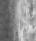
\includegraphics[width=0.19\columnwidth]{../images/thesis/okra/zoomed/weighted_prior_cropped.png}}
\caption[Zoomed results of Okra dataset]{Zoomed in portion corresponding to the red RoI of Fig.~\ref{fig:okra_3D_results} for various methods (b) has strong streak artefacts, (c) blurred, (d) no new  information detected (prior dominates -- the deformity from the prior
  shows up as a false positive) and (e) new information detected (no deformities
 ).}
\label{fig:okra_zoomed_3D_results}
\end{figure}

\end{document}
